% SPDX-FileCopyrightText: 2023 SAP SE
%
% SPDX-License-Identifier: Apache-2.0
%
% This file is part of FEDEM - https://openfedem.org

%%%%%%%%%%%%%%%%%%%%%%%%%%%%%%%%%%%%%%%%%%%%%%%%%%%%%%%%%%%%%%%%%%%%%%%%%%%%%%%%
%
% FEDEM Theory Guide.
%
%%%%%%%%%%%%%%%%%%%%%%%%%%%%%%%%%%%%%%%%%%%%%%%%%%%%%%%%%%%%%%%%%%%%%%%%%%%%%%%%

\section{Fatigue analysis}

Through fatigue analysis, one can asses the estimated life of a structural
component subjected to cyclic or repetitive loads, based on the computed
stress or strain history and some additional material properties.

The input to the fatigue analysis is the stress/strain reading in a virtual
strain gauge for each time step of the dynamics simulation,
\iftoggle{publicedition}{% The following is for the public edition
or alternatively one can compute the
{\em Signed absolute max\/} principal strain from the strain rosette tensor.
}{% The following is for the in-house edition only
\eqnref{eq:gage strain}, or alternatively one can compute the
{\em Signed absolute max\/} principal strain from the strain rosette tensor
given by \eqnref{eq:rosette strain}.
}% End in-house edition only
Letting $\{\varepsilon_1,\varepsilon_2\}$ denote the maximum and minimum
principal strains\footnote{These quantities are the same as the largest and
smallest eigenvalues of the symmetric strain tensor.}, respectively, the
signed absolute max value is defined through
%
\begin{equation}
\label{eq:signed abs max}
\varepsilon_\text{samax} \;=\; \left\{ \varepsilon_i :
|\varepsilon_i| = \max\{|\varepsilon_1|,|\varepsilon_2|\} \right\}
\end{equation}
%
Similarly, one can derive the signed absolute max principal stress,
$\sigma_\text{samax}$ from the stress tensor.
Using \eqnref{eq:signed abs max} will normally give a more conservative life
assessment compared to using a gauge leg reading, in cases where direction of
the maximum strain varies during the simulated event.
Using a gauge strain directly does not account for such variations.

\subsection{Peak valley extraction}

The first step in the process of obtaining the estimated life at a given point,
is to simplify the stress/strain history curve measured by the virtual strain
gauge, and removing oscillations smaller than a given threshold (gate value).
This is a process often referred to as {\em peak valley extraction\/}.

Consider the typical stress history reading, i.e., $\sigma_\text{samax}(t)$,
in Figure~\ref{fig:PVX}a), which typically consists of hundreds
(if not thousands) of data points.
In a life assessment, it is only the turning points of the curve that matter,
i.e., where the gradient of the curve changes sign.
Thus, after peak valley extraction using a gate value of 1 MPa,
the processed curve ends up as shown in Figure~\ref{fig:PVX}b).
The number of data points has been reduced from 201 to only 22 in this case.

\begin{figure}[b]
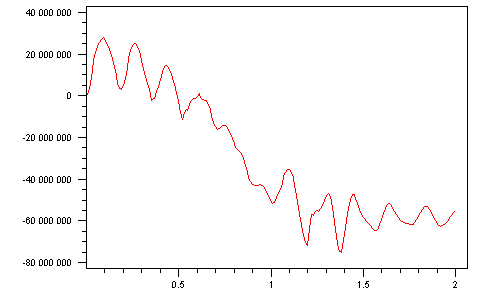
\includegraphics[width=0.5\textwidth]{Figures/LoaderRos9_sigma.png}
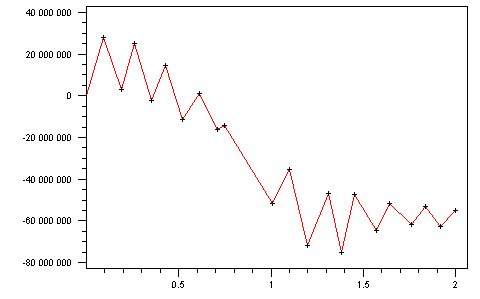
\includegraphics[width=0.5\textwidth]{Figures/LoaderRos9_pvx.png}
a) \hskip 0.5\textwidth b)
\caption{Peak valley extraction of a stress history curve.
a) The original stress curve.
b) The processed curve consisting of the turning points (+) only.}
\label{fig:PVX}
\end{figure}

\subsection{Rainflow analysis}

The next step of the fatigue analysis is to perform a {\em rainflow counting\/}
on the processed stress/strain signal, in order to further reduce a spectrum of
varying stresses/strains into a set of simple stress/strain reversals.
The process is named rainflow counting because it can be explained by viewing
the stress history curve like the one in Figure~\ref{fig:PVX}b) as a series of
Padoga roofs when it is rotated 90 degrees with the time axis vertically,
and letting drops of water flow from each peak and valley.
The stress cycles are then defined by how each flow of water is terminated
according to a set of rules.

In the algorithm adopted in Fedem, we traverse the peak and valley curve in
steps looking at three line segments defined by four neighboring points of the
curve (labeled 1, 2, 3, 4) in each step:
If the middle line 2-3 is shorter than both end lines 1-2 and 3-4, and its
gradient has opposite sign as the gradient of both lines 1-2 and 3-4, then
the points 2 and 3 define a full stress cycle and is removed from the curve.
We then proceed to the next step in which the previous point 4 becomes the
new point 2, while the subsequent two points in the curve become the new points
3 and 4.
If the points 2 and 3 were not removed, all four point counters are incremented
while proceeding to the next step.
We then continue until the entire curve has been traversed once.

The traversal is then restarted from the beginning of the curve, and
repeated until no more full cycles could be found during one traversal.
This process is illustrated in Figure~\ref{fig:Rainflow1} for the stress
curve of Figure~\ref{fig:PVX}, where we have encircled the full cycles detected
during the first traversal.
When these points are removed, the resulting curve becomes as shown in
Figure~\ref{fig:Rainflow2}a).

\begin{figure}[b]
\center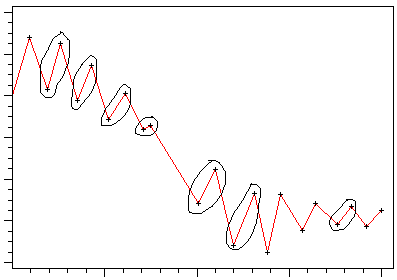
\includegraphics[width=0.84\textwidth]{Figures/LoaderRos9_pass0}
\caption{Rainflow analysis: Points defining full stress cycles detected
during the first traversal of the curve in Figure~\ref{fig:PVX}b).}
\label{fig:Rainflow1}
\end{figure}

\begin{figure}[t]
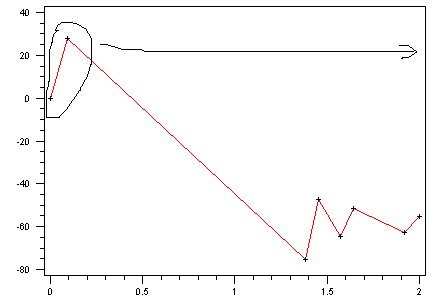
\includegraphics[width=0.5\textwidth]{Figures/LoaderRos9_pass1}
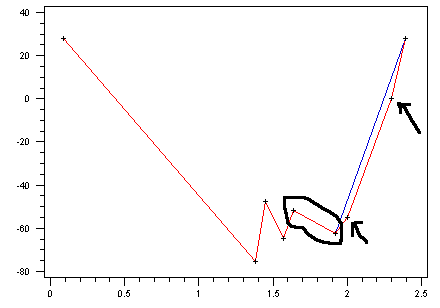
\includegraphics[width=0.5\textwidth]{Figures/LoaderRos9_pass2}
a) \hskip 0.5\textwidth b) \\[2mm]
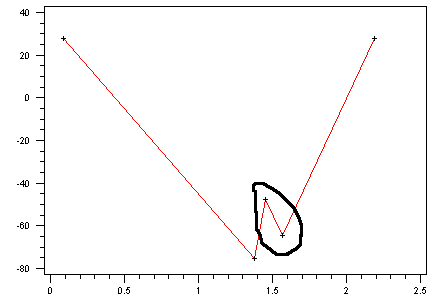
\includegraphics[width=0.5\textwidth]{Figures/LoaderRos9_pass3}
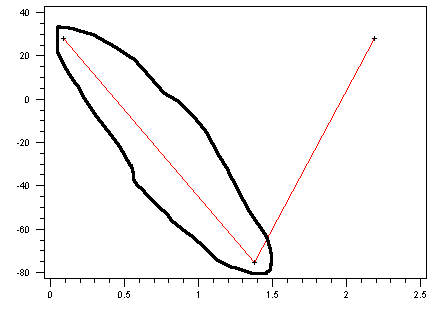
\includegraphics[width=0.5\textwidth]{Figures/LoaderRos9_pass4}
c) \hskip 0.5\textwidth d)
\caption{Subsequent steps of the rainflow analysis:
a) Inserting an additional max point making it the new start and end point.
b) Removing two `non-turning' points and the next full stress cycle.
c) Removing another full cycle in the next traversal.
d) Counting the final cycle.}
\label{fig:Rainflow2}
\end{figure}

Even when no more full cycles can be detected through the procedure outlined
above, there will normally still be some left-over points in the curve.
This is the situation already after the first traversal for the curve in
Figure~\ref{fig:Rainflow1}.
The remaining curve is then modified by duplicating the point with the largest
magnitude, and then shifting the added point and all preceding points to the
end of the curve, as illustrated by the arrow in Figure~\ref{fig:Rainflow2}a).
The modified curve then becomes as shown in Figure~\ref{fig:Rainflow2}b).
Here, the two points indicated by the arrows are not `turning points'.
They are therefore removed from the curve without counting a cycle, resulting
in the blue portion of the curve instead.
The traversal can now be repeated on the modified curve, until only three
points remain which then will count as the final cycle.
This process is depicted by the Figures~\ref{fig:Rainflow2}b-d),
where one cycle is detected in each traversal.

The rainflow counting outlined above can be performed in a similar manner for a
stress history and a strain history curve.
In Fedem it is only applied on stress history results.

\subsection{Damage and life calculation}

The rainflow analysis produces a list of stress ranges with magnitudes
$\bar{\sigma}_i$ representing the entire stress history in a given point for
the duration of the numerical simulation.
The accumulated damage in that point can now be computed using the S-N curve for
the material in question.

An S-N curve relates a stress range magnitude (S) to the number of repetitions
(N) of a cycle of that magnitude, a material point can sustain before failure.
S-N curves are typically derived from tests on samples of the material in
question, and may be found in various design codes for certain materials and
loading conditions.

For a given set of stress ranges, $\bar{\sigma}_i, i=1 \ldots k$, we read the
corresponding number of cycles before failure, $N_i$, from the specified
S-N, curve.
The accumulated damage is then computed as
%
\begin{equation}
C \;=\; \sum_{i=1}^k\frac{1}{N_i}
\end{equation}
%
and failure occurs when $C>=1.0$.
The estimated life in terms of number of repetitions of the simulated loading
event is then the reciprocal of this value, $1/C$.
If the simulated time span is denoted $T_s$, the estimated life at the
material point is therefore
%
\begin{equation}
\text{Life} \;=\; \frac{T_s}{C}
\end{equation}
